\subsection*{Nezapomenutelná návštěva}
\label{sub:nezapomenutelna_navsteva}

V rámci Lemuřího tábora jsme se krom příjemného pobývání v lůnu přírody, debužírování na našich gastronomických výtvorech a podnikání všelijakých skopičin snažili páchat i nějaké to dobro. Ostatně roverské heslo „sloužím“ nás k tomu přímo vybízelo. Proto když jsme zjistili, že v dochozí vzdálenosti od našeho tábořiště se nachází Domov Rakovice, místo pro široké spektrum lidí stižených některou z forem demence, neváhali jsme ani na moment a jali se navazovat s tímto ústavem kontakt. To se ukázalo být nečekaně komplikovanou procedurou. Na základě telefonického hovoru se slečnou sekretářkou se mi podařilo dohodnout schůzku s paní ředitelkou, což byla žena jako vystřižená z dámského časopisu a se svými vysokými podpatky, dlouhými nehty a parfémy zvučných značek tvořila až úsměvný protiklad k mému nemytému já.
To, co se mi prve jevilo jako prostý úkol – tedy vysvětlit, že jsme skauti, co chtějí přijít a povídat si se seniory, zahrát jim písničky a prostě tak nějak pobýt – se ukázalo být úkolem nečekaně náročným. Paní ředitelka nechápala, proč bychom to chtěli dělat, jaké jsme si pro ně připravili představení a kolik za to chceme peněz. Nicméně po vyjasnění, že to děláme pro radost, že s tím už nějaké zkušenosti máme, že nemáme představení, akorát ukulele, a že za to vážně nic nechceme, šokovaná paní ředitelka nabídku přijala pod jedinou podmínkou, a to že nám budou moci uvařit oběd. Proti tomu jsme nic neměli, pročež jsme se dohodli a o dva dny později do Rakovic ošátkováni dorazili.

Kromě vydatného oběda na nás čekaly dvě skupiny klientů, kterým jsme s velikým úspěchem hráli hitovky typu Hlídač krav, Lachtani nebo Nosorožec. Po dvou „koncertech“ jsme se rozdělili do menších skupinek a jali se věnovat klientům individuálně. Někteří z nás si jenom povídali, jiní hráli stolní hry nebo dělali ruční práce, a část z nás jela provézt výpravu vozíčkářů po vesnici. Asi nemá smysl zabíhat do přílišných podrobností, nicméně z celé návštěvy jsme odcházeli s neuvěřitelně pozitivním dojmem, protože klienti i personál byli extrémně přátelští a všechno se neslo v úžasně příjemném duchu. Holt jenom někde vzadu v mozku člověku hlodal pocit smutku, protože životní příběhy klientů byly často tragické, a zejména u (překvapivě velké) skupiny s alkoholovou demencí i docela výstražné.

No nakonec jsme v Rakovicích strávili celé odpoledne. Paní ředitelka nám přes protesty vtiskla do rukou bednu čokolády a peníze na zmrzlinu a hlavně vysvětlila, proč byli všichni z naší návštěvy tak zaskočení (a proč se naše úvodní domluva nesla v duchu nepochopení) – prý se jim ještě nikdy nestalo, že by za nimi do Domova přišel jen tak někdo na návštěvu…


\begin{center}

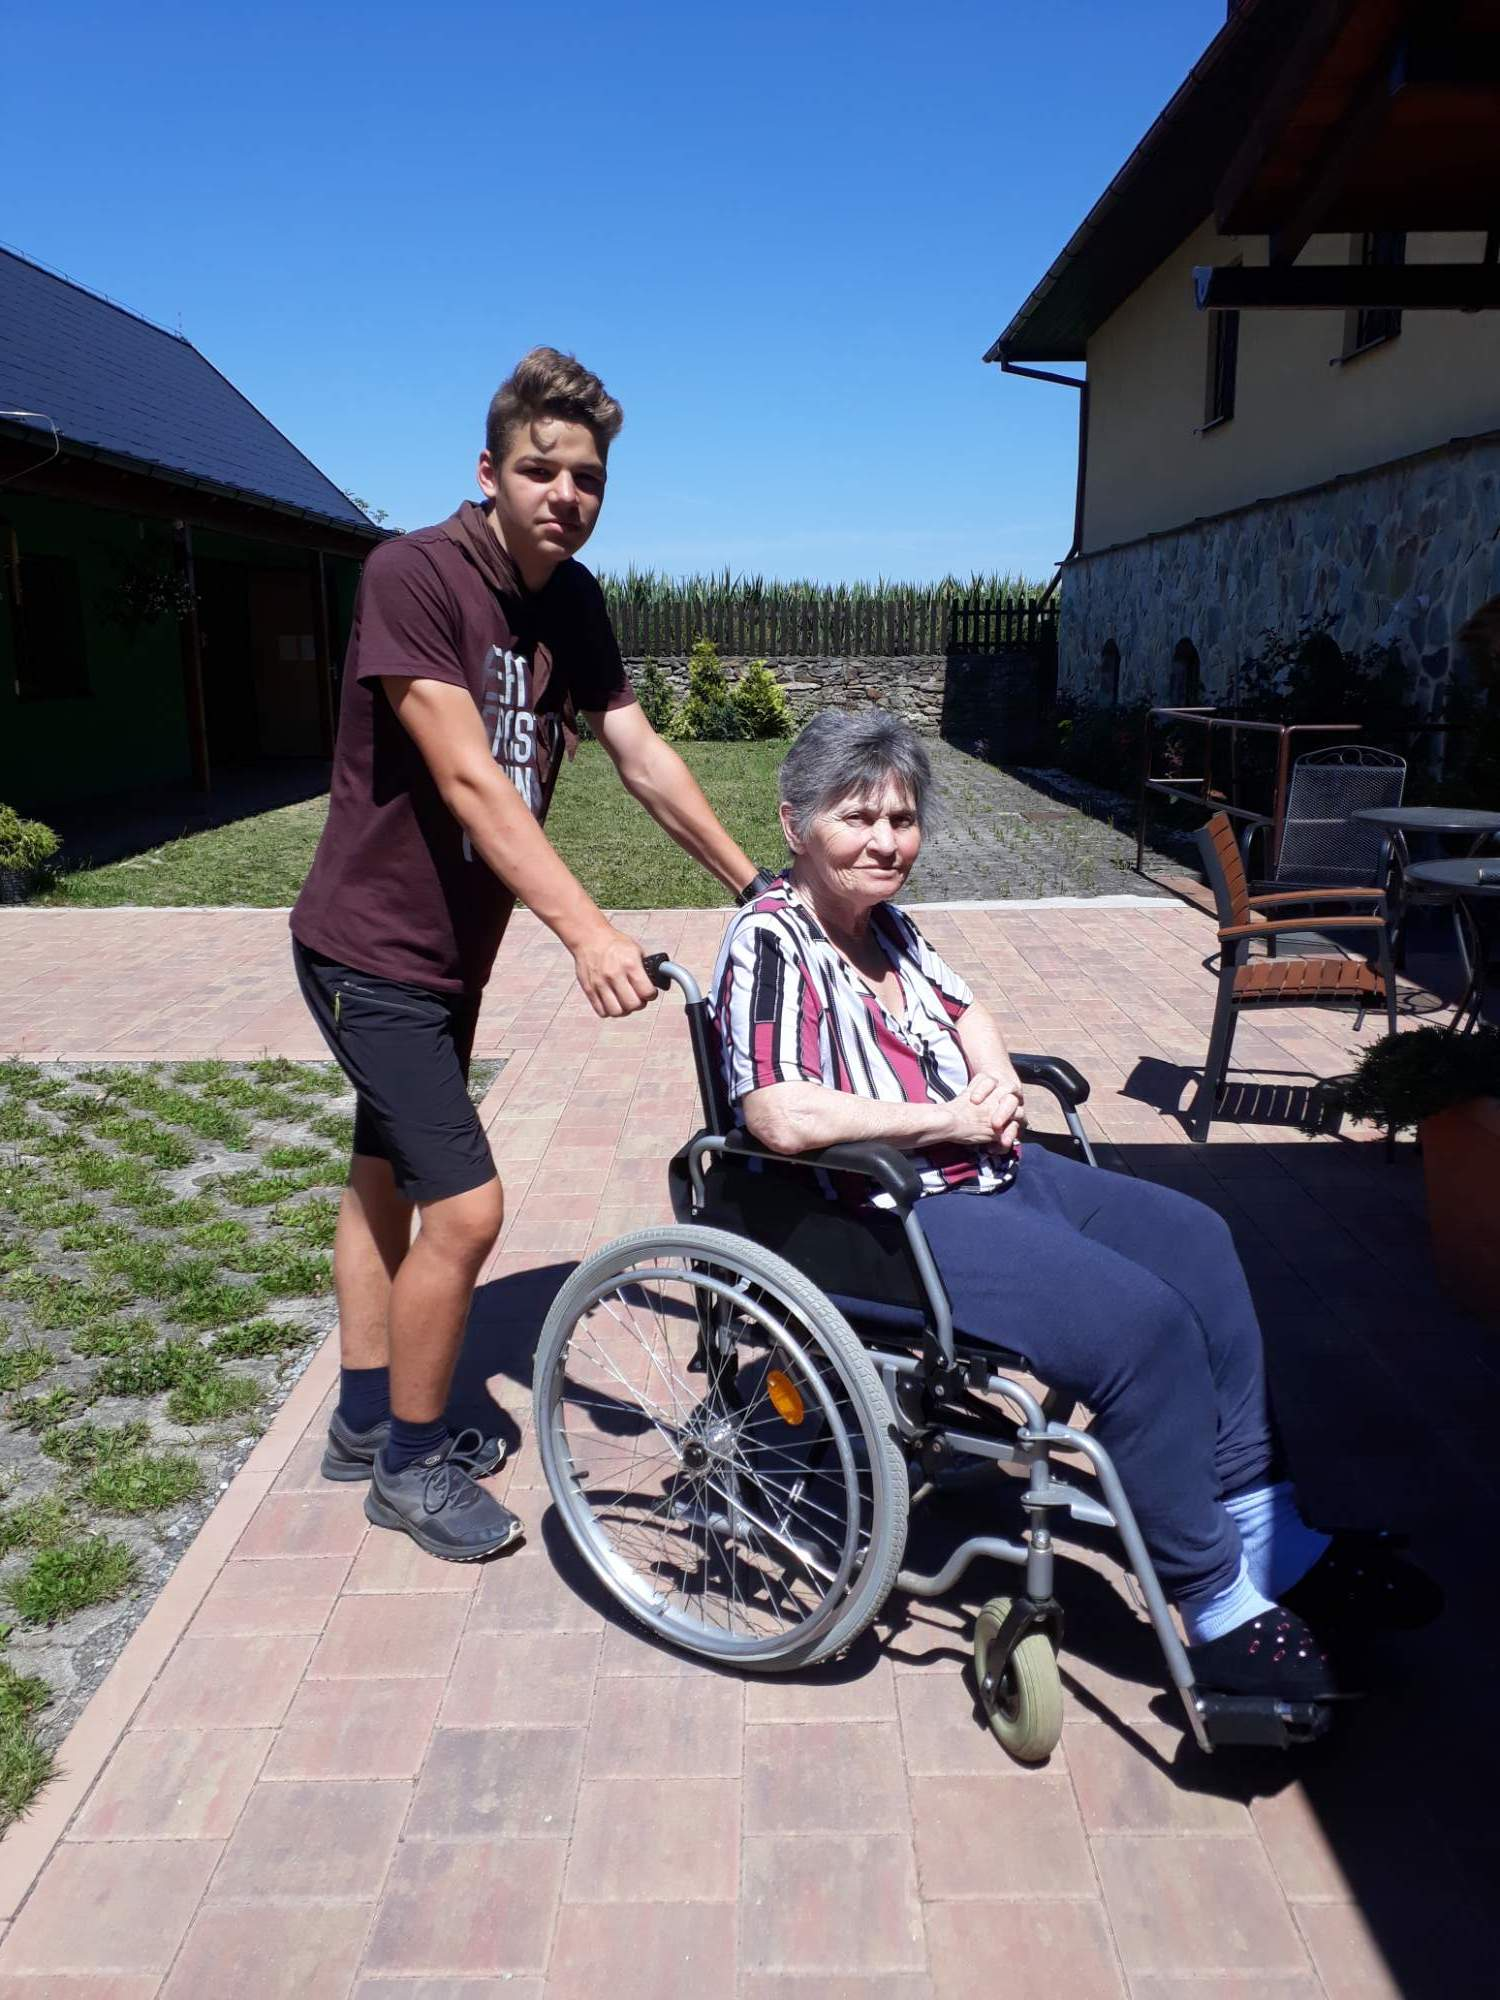
\includegraphics[width=4.5cm]{img/rovero_clanky/rizek_s_babou.jpg}

\end{center}

\podpis{Fík}